\AddToHook{package/hyperref/before}{\RequirePackage{float}}
\documentclass[pdflatex,iicol,sn-basic,Numbered]{sn-jnl}
\usepackage{graphicx,amsmath,amssymb,booktabs,tabularx,array,ragged2e,longtable}
\usepackage{tikz}
\usetikzlibrary{arrows.meta,positioning}
\usepackage{algorithm,algorithmicx,algpseudocode}
\usepackage{seqsplit,xurl}
\DeclareUnicodeCharacter{2212}{\ensuremath{-}}
\DeclareUnicodeCharacter{2192}{\ensuremath{\rightarrow}}
\DeclareUnicodeCharacter{00B1}{\ensuremath{\pm}}
\newcolumntype{L}[1]{>{\RaggedRight\arraybackslash\hspace{0pt}}p{#1}}
\newcolumntype{Y}{>{\RaggedRight\arraybackslash\hspace{0pt}}X}
\newcommand{\papertable}{\small\renewcommand{\arraystretch}{1.35}\setlength{\tabcolsep}{4pt}\emergencystretch=1em}
\newcommand{\sncstable}{\papertable}
\newcommand{\maintitle}{Preference-Graph Repair and Retrieval Utility: An Empirical Opportunity Audit}
\hypersetup{pdfauthor={Soroush Vahidi},pdfsubject={},pdfcreator={LaTeX},bookmarksdepth=2,colorlinks=true,linkcolor=black,citecolor=black,urlcolor=black}
\raggedbottom

% Fixed-position supplementary blocks retain ordinary numbered captions.
\makeatletter
\newenvironment{supplementtable}{\par\addvspace{10pt}\noindent\begin{minipage}{\linewidth}\def\@captype{table}}{\end{minipage}\par\addvspace{10pt}}
\makeatother

\ifdefined\AnonymousVersion\hypersetup{pdfauthor={}}\fi
\urlstyle{same}
\emergencystretch=1em

\hypersetup{pdftitle={Preference-Graph Repair and Retrieval Effectiveness: An Empirical Decomposition}}

\begin{document}
\title[Preference-Graph Repair and Retrieval Effectiveness]{\maintitle}
\ifdefined\AnonymousVersion
\author{\fnm{Anonymous} \sur{manuscript}}
\else
\author*[1]{\fnm{Soroush} \sur{Vahidi}}\email{sv96@njit.edu}
\affil*[1]{\orgdiv{Department of Computer Science}, \orgname{New Jersey Institute of Technology}, \orgaddress{\city{Newark}, \state{New Jersey}, \country{USA}}\\ORCID: \href{https://orcid.org/0000-0003-1934-6282}{0000-0003-1934-6282}}
\fi

\abstract{Preference-graph repair removes contradictory comparisons, but structural consistency and retrieval effectiveness are different objectives. Their separation is well understood in principle; less clear is where the effect of repair stops between the graph, the extracted ranking and its evaluated relevance profile. We investigate this question through matched unrepaired, greedy and exact-repair comparisons that hold candidates, preference evidence, extraction and evaluation fixed. The central analysis decomposes responses on 213 selected queries across four datasets. Greedy and exact repair change 180 and 160 rankings, respectively, yet measured utility remains unchanged in 79.4\% and 84.4\% of those changed rankings. Two mechanisms account for these zeros: pools without a judged-positive candidate and positive-containing pools whose evaluated top-ten relevance profile is preserved. The latter occurs in 74 cases per repair branch and across every dataset and provider-availability stratum. Thus missing judged opportunity alone does not explain the observed inactivity. Query-block inference supplies no Holm-adjusted rejection in the 35 exact-versus-greedy comparisons, while a complete small-instance diagnostic shows that equal-cost repairs can yield different utility. These findings distinguish an intervention that changes rankings from one that changes measured relevance. They extend earlier construction-dependent evidence through conditional frequencies and relevance-profile attribution, rather than a new repair algorithm. Nonrandom selection, incomplete judgments, sparse informative support and an unreliable compact-model comparison instrument limit generalization; the results establish neither equivalence nor a universal absence of benefit.}
\keywords{preference graphs, feedback arc set, graph repair, rank aggregation, information retrieval, retrieval evaluation}
\maketitle

\section{Introduction}\label{sec:introduction}
Pairwise comparisons offer a flexible way to rank documents using evidence from several retrieval models or language-model judges. A comparison favoring document $u$ over $v$ becomes a directed edge $u\to v$. Aggregated comparisons can form cycles, making it impossible to satisfy every preference in one order. Removing a feedback arc set resolves that structural contradiction. It does not, however, determine whether a relevant document moves to a better position. The graph objective concerns agreement with the comparisons; retrieval effectiveness concerns relevance to the query.

This distinction creates an evaluation problem. A small average retrieval effect can arise because the graph requires no repair, because deletion leaves the extracted order unchanged, because a changed order preserves the relevance grades seen by the metric, or because gains and harms offset one another. These outcomes have different implications. The first offers little opportunity to assess deletion, the second depends on the extractor's response, and the third concerns which ranking changes the evaluation can distinguish. A mean effect alone does not locate that separation.

Existing research establishes effective pairwise and graph-based ranking methods, and our public preprint already reports construction-dependent cyclicity and conditional retrieval effects \cite{vahidi2026retrievalpreprint}. The unresolved empirical question is how often structural interventions reach the ranking and measured-relevance stages, and how the resulting zeros are distributed across the observed query populations. Equal evaluated grade sequences necessarily give equal nDCG under fixed normalization; that identity does not tell us whether such cases are common, whether they contain judged-positive candidates, or whether a few datasets dominate them.

We ask: \emph{when preference-graph repair improves structural consistency, under what observed conditions does it change the extracted ranking and measured retrieval effectiveness?} We compare unrepaired, greedy and exact-repair branches while holding candidates, comparison evidence, extraction, tie handling and evaluation fixed. Four score-derived benchmarks provide controlled construction contrasts; a selected multi-provider cohort supports complete ranking and relevance-profile attribution. A six-query diagnostic examines all minimum-cost repairs, and a separate compact-model cohort tests the limits of the elicited evidence. These cohorts have different selection and measurement conditions and are not interchangeable replications.

\subsection{Scientific contributions}
The principal contribution is an empirical decomposition of the response to graph repair:
\begin{enumerate}
\item \textbf{From graph modification to ranking response.} We distinguish acyclic inputs from cyclic graphs whose repair leaves the fixed extractor's ranking unchanged (Section~\ref{sec:opportunities}).
\item \textbf{From ranking response to measured relevance.} On 213 selected queries, complete relevance-profile attribution separates changed rankings without judged-positive candidates from changed positive-pool rankings with fixed evaluated profiles. Dataset and provider-availability composition shows where these mechanisms occur, with both gains and harms retained (Section~\ref{sec:profiles}).
\item \textbf{From structural optimality to utility ambiguity.} Complete optimum sets for six graphs quantify the utility variation left unidentified by minimum deletion cost under fixed extraction (Section~\ref{sec:optimum-choice}).
\end{enumerate}
These are analyses of reused observations, not new independent datasets. Graph-repair algorithms and ranking--MWFAS theory are established methods. Corrected query-block inference supports the interpretation of the results; computational verification checks their arithmetic and finite completeness. Neither correction nor verification is presented as algorithmic novelty. The scientific increment is the observed composition of the intervention's responses, which distinguishes missing evaluated opportunity from active ranking changes that measured relevance does not distinguish.

\section{Related Work}\label{sec:related}
\subsection{Preference aggregation and structural objectives}
Classical rank aggregation reconciles inconsistent preferences through minimum-disagreement ordering and related objectives \cite{dwork2001rank,ailon2008aggregating}. Feedback arc set optimization and linear-ordering formulations provide established methods for removing cycles \cite{groetschel1984cutting,baharev2021exact}. The author's earlier training-free ranking pipeline develops the ranking--feedback-arc relationship and combines pruning, cycle-safe add-back and refinement \cite{vahidi2026acyclicranking}. Those methods, theory and ranking-recovery results are prior work. Related structural graph-benchmark research concerns graph identity and comparisons among existing optimizers; its benchmark outcomes are not new retrieval observations in the present study. Our question instead concerns deletion's effect against external relevance judgments.

Alternative aggregation methods infer an order without solving a deletion problem. Bradley--Terry models estimate latent strengths \cite{bradley1952rank,hunter2004mm}; Rank Centrality uses a comparison Markov chain \cite{negahban2017rankcentrality}; combinatorial Hodge theory separates ranking and cyclic components of pairwise flow \cite{jiang2011hodge}. SpringRank estimates a hierarchy through a weighted quadratic energy \cite{debacco2018springrank}, while reciprocal rank fusion combines source ranks without constructing a preference graph \cite{cormack2009rrf}. These methods motivate complementary controls, but changing the aggregator as well as repairing the graph does not isolate deletion's contribution. Nor do their assumptions make arbitrary edge weights calibrated correctness probabilities.

\subsection{Language-model ranking and retrieval evaluation}
Pairwise ranking prompting uses language-model comparisons to rerank documents \cite{qin-etal-2024-large}. PRP-Graph incorporates target-label probabilities into graph construction and aggregation \cite{luo2024prpgraph}; a winner-only cache cannot recover that probability information. Listwise and setwise prompting elicit different evidence by ordering or selecting among several documents jointly \cite{sun-etal-2023-chatgpt,zhuang2024setwise}. Our adapted PRP-Graph comparison therefore provides pipeline context rather than an exact reproduction of published effectiveness or an isolated test of edge deletion.

LLM-RankFusion addresses presentation-order and transitive inconsistency through prompting, calibration and aggregation \cite{zeng2026llmrankfusion}. Preference Graph Ensemble and Denoise uses multiple evaluators to obtain acyclic judgments for model evaluation, response selection and training-data selection \cite{hu2026acyclic}. TourRank combines tournament-style grouping with a points-based ensemble for document ranking \cite{chen2025tourrank}. Xu et al. show that nontransitive judgments can make model rankings sensitive to the baseline, and study tournament acquisition with Bradley--Terry aggregation \cite{xu2025nontransitivity}. These studies establish the relevance of consistency and its mitigation under their own tasks and acquisition procedures. They do not determine whether minimum-weight deletion improves document relevance when evidence and extraction are held fixed.

The distinction between intrinsic consistency and task-dependent quality is established in data-quality research \cite{wang1996beyond}. Likewise, nDCG measures relevance at ranking positions rather than agreement with comparison edges \cite{jarvelin2002cumulated}. Buckley and Voorhees examine retrieval evaluation with incomplete relevance information \cite{buckley2004incomplete}, motivating the distinction between an evaluation zero and semantic irrelevance. Their work does not validate our selected cohorts or recover their unobserved relevance. We retain the original metric definitions rather than select a different metric after observing zeros.

The public retrieval preprint already distinguishes construction, repair and extraction \cite{vahidi2026retrievalpreprint}. The present analysis adds complete selected-cohort attribution, its dataset and provider-availability composition, and the finite all-optimum diagnostic. Online Resource~1 identifies reused records and construction/normalization differences; the legacy-to-current execution bridge remains incomplete. Corrected paired inference respects independent query units and multiplicity \cite{urbano2019statistical,carterette2012multiple}. A failure to reject still does not establish equivalence \cite{lakens2018equivalence}. These inferential qualifications support the empirical contribution without turning reused evidence into independent replication.

\section{Problem Formulation}\label{sec:problem}
\subsection{Fixed-evidence repair contrast}
For query $q$, let $D_q$ be a fixed candidate set and $G_q=(D_q,E_q,w_q)$ its directed preference graph. Edge $u\to v$ favors placing $u$ ahead of $v$; its nonnegative weight represents recorded evidence strength, not ground-truth relevance. A feedback arc set $F$ makes $G_q-F$ acyclic. Minimum-weight repair solves
\begin{equation}
\begin{aligned}F_q^\star&\in\arg\min_{F\subseteq E_q}\sum_{e\in F}w_q(e)\\
&\text{subject to }G_q-F\text{ being acyclic}.\end{aligned}
\label{eq:mwfas}
\end{equation}
The empty deletion is optimal for an acyclic positive-cost graph. Acyclicity need not imply a unique total order or relevance-optimal preferences. A structural optimum need not identify a unique deletion set either.

Let $\mathcal R$ denote a fixed deterministic ranking extractor and $U_q$ the retrieval metric with fixed relevance judgments and normalization. For a returned repair $F$, the observed contrast is
\begin{equation}
\Delta_q(F)=U_q\!\left(\mathcal R(G_q-F)\right)-U_q\!\left(\mathcal R(G_q)\right).
\label{eq:contrast}
\end{equation}
Greedy, exact and unrepaired branches share these inputs. An exact certificate concerns Eq.~\eqref{eq:mwfas}, not the maximum of Eq.~\eqref{eq:contrast}. It also does not characterize every equally optimal repair or all rankings obtainable from a repaired graph.

\subsection{Rankings, relevance and opportunity stages}
The principal extractor for cached judgments is unweighted Copeland: outgoing degree minus incoming degree, sorted in descending order with ascending document-ID ties. The score-derived studies also hold other extractors fixed within their repair contrasts. Some extractors can be applied to cyclic graphs; topological extraction requires a directed acyclic graph (DAG) and appears only in suitable repaired-graph comparisons. Acyclicity alone does not guarantee that a score-based extracted order respects every retained edge.

Let $\pi_q=(d_1,\ldots,d_{P_q})$ rank the fixed candidates, and let $r_q(d)$ be the recorded relevance grade, with an unjudged candidate assigned evaluation grade zero. Define $k_q=\min(k,P_q)$. Normalized discounted cumulative gain is
\begin{equation}
\operatorname{nDCG}_q@k=
\frac{\sum_{i=1}^{k_q}(2^{r_q(d_i)}-1)/\log_2(i+1)}{\operatorname{IDCG}_q@k}.
\label{eq:ndcg}
\end{equation}
For an ideal-reference set $B_q$, let $r^\downarrow_{q,B_q,i}$ denote its grades sorted in descending order. Ideal discounted cumulative gain (IDCG) is
\begin{equation}
\operatorname{IDCG}_q@k=\sum_{i=1}^{\min(k,|B_q|)}
\frac{2^{r^\downarrow_{q,B_q,i}}-1}{\log_2(i+1)}.
\label{eq:idcg}
\end{equation}
The implementation returns zero when IDCG is nonpositive. Candidate-conditioned IDCG uses $B_q=D_q$; full-query IDCG uses the complete recorded query qrels, including judged documents outside the candidate pool. Thus a short candidate ranking does not truncate the full-query ideal to the pool size. Evaluation zeros for unjudged documents do not establish irrelevance.

For binary relevance $z_{qi}=\mathbf1\{r_q(d_i)>0\}$ and $R_q=\sum_{i=1}^{P_q}z_{qi}$, the historical exact-versus-greedy endpoints are
\begin{equation}
\begin{aligned}\operatorname{AP}_q&=\frac{1}{R_q}\sum_{i=1}^{P_q} z_{qi}\frac{\sum_{j=1}^{i}z_{qj}}{i},\\
\operatorname{RR}_q&=\frac{1}{\min\{i:z_{qi}=1\}}.\end{aligned}
\label{eq:ap-rr}
\end{equation}
Both are defined as zero when $R_q=0$. Average precision (AP) and reciprocal rank (RR) use the complete recorded candidate ranking, not the full corpus. Within a single cell, mean average precision (MAP) and mean reciprocal rank (MRR) are the arithmetic means of AP and RR over eligible queries; the historical MAP label does not change AP's candidate-positive denominator. Within a fixed comparison, methods share candidates, labels, cutoff and IDCG. Across families, changing IDCG can rescale query effects and their aggregate weighting; the original contracts are retained.

We distinguish graph modification, full-ranking response and evaluated grade-position response. If a changed ranking has the same first-$k$ grade sequence and fixed IDCG, Eq.~\eqref{eq:ndcg} is unchanged. This is a sufficient explanation for a recorded zero; different grade sequences can also yield equal metric values. Top-$k$ membership is a separate diagnostic: reordering a fixed set can change nDCG, while exchanging equal-gain documents can preserve it. We therefore do not use membership change as a necessary gate for retrieval activity.

\section{Experimental Design}\label{sec:design}
\subsection{Datasets and query populations}
Table~\ref{tab:cohorts} separates the evidence populations. We use relevance judgments (qrels) as the external evaluation reference. The canonical score-derived study uses SciDocs, FiQA, HotpotQA and BRIGHT \cite{cohan2020scidocs,maia2018fiqa,yang2018hotpotqa,su2025bright}. These benchmarks provide heterogeneous relevance supervision, including citation- and question-answering-derived labels. They are not uniformly direct human pairwise gold standards. Newer FiQA and SciDocs cohorts use BEIR-hosted snapshots \cite{thakur2021beir}; the historical HotpotQA retrieval conversion remains incompletely pinned.

\begin{table*}[t]
\caption{Evidence cohorts and comparison contracts. Counts are unique query identities within each row; rows are not an additive independent sample. C/F denote candidate-conditioned/full-query IDCG.}
\label{tab:cohorts}\papertable
\begin{tabularx}{\linewidth}{@{}L{2.25cm}rL{2.25cm}Y@{}}\toprule
Cohort & Queries & Pool / IDCG & Selection and role \\\midrule
Score-derived &342&20 or 10; larger 50 or 35 / C, F&Stored multi-ranker scores; 1,025 repeated query--regime exact instances; C for repair--unrepaired, F for pooled exact--greedy; details in Section~\ref{sec:statistics} \\\addlinespace
Cached primary &6&8 / F&Qrel-enriched four-provider diagnostic; complete optimum envelope \\\addlinespace
Selected cache &213&15 / F&Retrospective provider-availability strata: 110 two-provider and 103 four-provider aggregates \\\addlinespace
PRP-Graph pilot &20&20 / F&10 FiQA, 10 SciDocs; adapted external acquisition/aggregation comparison \\\addlinespace
Prospective &20&12 / F&7 FiQA, 7 SciDocs, 6 BRIGHT; two compact models, strict repair contrasts \\\addlinespace
Candidate diagnostic &20&12 per arm / F&Further queries; BM25 versus BGE selection from BM25 top 100 \\\bottomrule
\end{tabularx}
\end{table*}

Canonical counts are 120 SciDocs, 120 FiQA, 52 HotpotQA and 50 BRIGHT queries. Eighteen of 70 stored HotpotQA queries fail the canonical relevant-candidate eligibility condition. The six-query primary cache is disjoint from the selected 213-query cache; the latter comprises 77 SciDocs, 76 FiQA, 42 BRIGHT and 18 HotpotQA identities. It is selected and heterogeneous rather than a random prospective replication. Seventy-nine selected-cache pools have no judged-positive candidate; they remain in principal means.

The three newer 20-query cohorts are mutually disjoint. BGE reuses the PRP and prospective pools; graph-construction variants and prompt development reuse the prospective queries. The prospective collection contains 5,880 responses, but only 20 query units. Online Resource~1 preserves cohort selection, snapshot and reuse details.

\subsection{Construction, repair and extraction contracts}
The canonical graph uses stored BM25 lexical-retrieval scores, term frequency--inverse document frequency (TF-IDF) scores and MiniLM sentence-encoder scores as a controlled multi-source substrate. Per-query, per-ranker min--max normalization precedes margin votes. Retention-matched thresholds depend on stored score distributions, not relevance labels, but are calibrated on the evaluated query list and are therefore transductive. The permissive \texttt{ms1} rule retains ranker-supported directions; \texttt{ms2} requires support from at least two of three rankers; \texttt{ms1\_drop\_mutual} removes contested pairs during construction. This last rule differs from deleting reciprocal edges from an already constructed graph. Candidates come from the fixed reciprocal-rank-fusion pool policy; full thresholds and alternative policies are in Online Resource~1.

For cached judgments, strict parsing accepts complete A/B choices, maps reversed presentations back to document identity, and retains a provider edge only when both valid orientations agree. AB denotes the original document presentation and BA its reversal. Invalidity, abstention and reversal conflict never become a default winner. Individual-provider edges have unit weight; the primary aggregate sums contributions of one quarter per provider, preserving opposing directions. All candidates, including isolates, remain nodes. Prospective Qwen2.5-7B-Instruct (7 billion parameters) and SmolLM3-3B (3 billion parameters) judgments use a separately frozen JSON protocol; strict construction similarly requires agreement of valid directional responses. Confidence labels are not calibrated probabilities. Alternative constructions are exploratory repeated views, not selected replacements for the strict protocol.

Greedy repair repeatedly deletes a minimum-weight edge from a deterministic depth-first-search cycle until acyclic. It is not the Eades--Lin--Smyth ordering heuristic \cite{eades1993heuristic}. Exact repair uses a linear-ordering mixed-integer program solved by SCIP through PySCIPOpt \cite{achterberg2009scip,maher2016pyscipopt}, requiring proven optimality with zero reported gap. Pool, evidence, extractor, ties and cutoff remain fixed within a contrast, as shown in Fig.~\ref{fig:pipeline}. The complete six-query diagnostic enumerates all distinct optimal deletion sets with independent completeness checks; it is conditional on six eight-node graphs, not a new optimizer.

\begin{figure*}[t]
\centering
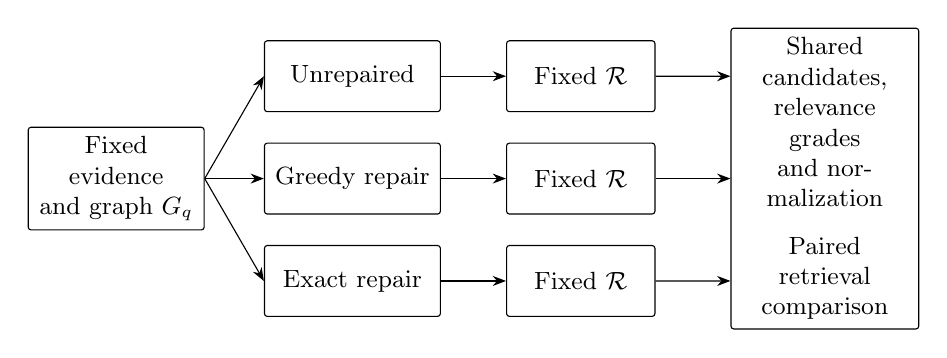
\begin{tikzpicture}[>=Stealth,font=\small,box/.style={draw,rounded corners=1pt,align=center,minimum height=0.9cm,text width=2.0cm},x=1cm,y=1cm]
\node[box] (g) at (0,0) {Fixed evidence\\and graph $G_q$};
\node[box] (u) at (3,1.3) {Unrepaired};
\node[box] (h) at (3,0) {Greedy repair};
\node[box] (e) at (3,-1.3) {Exact repair};
\node[box,text width=1.65cm] (eu) at (5.9,1.3) {Fixed $\mathcal R$};
\node[box,text width=1.65cm] (eh) at (5.9,0) {Fixed $\mathcal R$};
\node[box,text width=1.65cm] (ee) at (5.9,-1.3) {Fixed $\mathcal R$};
\node[box,minimum height=3.5cm,text width=2.15cm] (metric) at (9,0) {Shared candidates,\\relevance grades\\and normalization\\\medskip Paired retrieval\\comparison};
\draw[->] (g.east)--(u.west);\draw[->] (g.east)--(h.west);\draw[->] (g.east)--(e.west);
\draw[->] (u)--(eu);\draw[->] (h)--(eh);\draw[->] (e)--(ee);
\draw[->] (eu.east)--([yshift=1.3cm]metric.west);\draw[->] (eh.east)--(metric.west);\draw[->] (ee.east)--([yshift=-1.3cm]metric.west);
\end{tikzpicture}

\caption{Matched repair comparison. Each branch uses the same deterministic extractor $\mathcal R$, candidate set, tie handling, relevance grades, evaluation cutoff and normalization. Only graph repair changes; alternative aggregation methods are separate controls}
\label{fig:pipeline}
\end{figure*}

External comparisons include original-graph SpringRank, direct Bradley--Terry-style aggregation, graph-free fusion, adapted PRP-Graph and a trained BGE cross-encoder. BGE follows the official raw-relevance-logit procedure on matched documents \cite{bge2024modelcard}; it is not budget- or training-matched to a generative comparator. The adapted PRP pilot retains the published implementation's Swiss comparisons and personalized PageRank, but changes local pooling and runtime orchestration. It is not an exact reproduction of the published retrieval experiment. Missing or invalid listwise outputs remain missing controls. These distinctions prevent an acquisition or extractor change from being attributed to edge deletion.

\subsection{Evaluation and query-level inference}\label{sec:statistics}
The greedy-versus-unrepaired 20/60/110 and exact-versus-unrepaired 36/56 families use candidate-conditioned nDCG. Canonical cutoffs equal pool size: 20 for SciDocs, FiQA and BRIGHT, and 10 for HotpotQA. The larger-pool study retains its recorded $(P,k)$ cells, including $P=k$ reference cells. The historical exact-versus-greedy 35/399 families instead use full-query IDCG at eligible cutoffs 5, 10 and 20; their MAP and MRR use complete candidate rankings. Cached/prospective LLM, SpringRank, PRP-Graph, BGE and candidate-coverage results use full-query nDCG@10. These families' absolute means are not directly interchangeable. Online Resource~1 provides the endpoint/family map.

The corrected 35-test family crosses seven fixed extractors---balance, balance hybrid, Copeland, Copeland hybrid, damped Markov, topological and priority-topological---with MAP, MRR and the three nDCG cutoffs. The independent unit is the dataset--query identity, conditional on the benchmark sampling assumptions. Within a repair-versus-unrepaired cell, inference uses one paired query effect. In the separate pooled exact-versus-greedy diagnostic, repeated construction regimes form one dependent query block. Ordinary single-cell means weight eligible queries equally. The pooled diagnostic retains its original regime-row-weighted effect rather than silently substituting an equal-query average. For query sums $S_q$ and eligible regime counts $m_q$, its statistic is
\begin{equation}
T=\frac{\sum_q S_q}{\sum_q m_q},\qquad
S_q=\sum_{r\ \mathrm{eligible}}\bigl(U_{qr}^{\mathrm{exact}}-U_{qr}^{\mathrm{greedy}}\bigr).
\label{eq:pooled}
\end{equation}
There are 342 query units for 28 comparisons and 290 for seven nDCG@20 comparisons, which exclude the original ineligible HotpotQA cutoff. Their 1,025 and 869 eligible regime rows, respectively, are not independent observations. The historically omitted empty BRIGHT/\texttt{ms2} record remains excluded, without zero imputation.

The query-block analysis uses 10,000 Monte Carlo whole-query sign assignments, seed 17, add-one two-sided p-values, and Holm correction over the unchanged 35-test family \cite{holm1979simple}. Bootstrap sensitivity uses 10,000 within-dataset query-cluster draws, seed 13, with percentile and basic 95\% intervals. This corrected family does not use exact enumeration or bias-corrected and accelerated (BCa) intervals. All original effect estimates are preserved; historical row-based p-values are superseded.

Sign-flip inference assumes independent query units and exchangeability of the entire query's exact/greedy outcome vector under label swap. Mean zero alone does not justify that null, and the deterministic methods were not randomly assigned. Bootstrap intervals are approximate and pointwise, especially with sparse, skewed differences. Separate canonical, larger-pool, 399-cell and exploratory families retain their own procedures and error scope; their juxtaposition provides no global error guarantee. In model-averaged prospective contrasts, fixed-model effects are averaged within query before inference; model-specific comparisons retain one effect per query. Nonsignificance is not equivalence, and a pointwise interval does not override a Holm decision. Online Resource~1 provides the complete comparison families and inference details.

\subsection{Computational methods and AI assistance}\label{sec:evidence-access}
The analyses use fixed comparison evidence and deterministic extraction within each repair contrast. Online Resource~1 specifies runtime versions, thresholds, model settings and numerical verification procedures. Historical hosted-model aliases and incomplete scorer reconstruction constrain computational reproducibility; data and code access are described in the declarations.

Anthropic Claude and OpenAI ChatGPT/Codex assisted with software development, analysis utilities, figures and drafting. The author retains responsibility for verifying the text, code, analyses and citations against the underlying evidence. These tools are not authors.

\section{Structural and Ranking Opportunities}\label{sec:opportunities}
\subsection{Construction-dependent cyclicity}
Table~\ref{tab:opportunities} distinguishes graph workload from query support. Of 1,025 canonical graph records, 646 are acyclic and 379 cyclic. The records reuse 342 queries across three regimes; 316 identities are cyclic under at least one regime. Conservative \texttt{ms2} graphs are acyclic throughout the observed cohort. This is an empirical property of these constructed inputs, not a theorem that majority-supported preferences are always acyclic.

In the active \texttt{ms1} regime, cyclic-query rates are 99.2\% for SciDocs, 98.3\% for FiQA, 63.5\% for HotpotQA and 92.0\% for BRIGHT. Construction-time mutual dropping reduces them to 11.7\%, 30.8\%, 1.9\% and 22.0\%. Post-hoc reciprocal deletion from the SciDocs \texttt{ms1} graph instead gives 10.8\%; the different operation and threshold contract matter. Source-scale sensitivity is also substantial: conditional BM25 edge-weight share is 0.988 under raw margins and 0.512 after normalization. These measurements establish construction dependence, not the semantic accuracy of the resulting votes.

\begin{table*}[t]
\caption{Structural and ranking opportunity. Greedy/exact outcomes share queries. A dash denotes an unavailable complete ranking decomposition, not zero activity}
\label{tab:opportunities}\papertable
\begin{tabularx}{\linewidth}{@{}Yrrrr@{}}\toprule
Cohort & Query IDs & Graph records & Cyclic & Cyclic, same rank G/E \\\midrule
Canonical &342&1,025&379&---\\\addlinespace
Selected cache &213&213&191&11 / 31\\\addlinespace
Strict prospective &20&40&1&0 / 0\\\bottomrule
\end{tabularx}
\smallskip\small
Canonical records repeat construction regimes. Prospective records repeat two models; its sole cyclic graph has no judged-positive candidate. Both repairs modify every reported cyclic input graph; the extracted ranking can remain unchanged.
\end{table*}

The genuine-judgment cohorts demonstrate a separate aggregation effect. All 24 individual-provider graphs in the six-query corrected pilot are acyclic, but all six four-provider aggregate graphs are cyclic. In the selected cache, the two disjoint provider-availability strata contain 89/110 and 102/103 cyclic aggregate graphs. Absence of structural opportunity therefore cannot explain the selected-cache outcomes generally.

The prospective strict protocol has no cyclic-positive case: only one of 40 model/query graphs is cyclic, and its candidate pool contains no judged-positive document. All 14 positive-containing model/query graphs are acyclic. The alternative constructions create more cycles but reuse the same 20 queries. Qwen cyclic counts for strict, AB-only, BA-only, symmetric-both-valid and symmetric-available rules are 0/8/8/5/5; Smol counts are 1/13/12/1/5. More retained edges change the intervention opportunity, without establishing more reliable preference evidence.

\subsection{Repair activity and ranking response}
Both repairs modify all 379 cyclic canonical records and all 191 selected-cache cyclic aggregates. Exact repair has a different deletion set from greedy in 87.9\% of canonical cyclic records. It strictly lowers removed weight in 333 of those 379 records; lower dataset-mean removal costs are shown in Fig.~\ref{fig:cost}. Mean reductions relative to greedy are 25.1\%, 29.2\%, 13.4\% and 22.3\% for SciDocs, FiQA, HotpotQA and BRIGHT. These are structural quantities; retrieval effect sizes are evaluated separately.

\begin{figure*}[t]
\centering
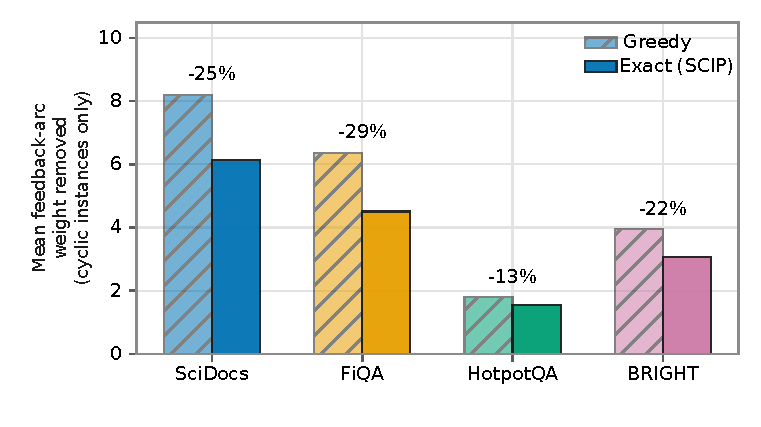
\includegraphics[width=\linewidth]{Fig2.pdf}
\caption{Mean deletion weight on 379 cyclic canonical query--regime records, pooled over ms1, ms2 and construction-time mutual dropping. Hatched/solid bars denote greedy/exact repair. Percentage labels show the original rounded reduction from the greedy dataset mean; individual records can tie. These are structural costs, not retrieval effects}
\label{fig:cost}
\end{figure*}

Graph activity does not imply a full-ranking response. Among the 191 cyclic selected-cache graphs, greedy leaves 11 Copeland rankings unchanged and exact leaves 31 unchanged. Including 22 acyclic graphs, unchanged-ranking totals are 33 and 53 of 213. This difference shows that choosing a structurally cheaper deletion can change the amount of extracted-order activity; it is not evidence that activity itself is beneficial. In the six-query aggregate diagnostic, each repair changes two rankings and leaves four unchanged.

The prospective construction workload contains 400 greedy/exact branch records across 200 model/query/construction graphs. Existing diagnostics identify 116 graph changes, 106 ranking changes and nine nonzero utility records, covering six query identities. These workload counts are descriptive repeated measurements of 20 queries. Complete historical permutations are unavailable for the 1,025 historical exact canonical scalar records, so a corresponding full canonical rank-response decomposition is not reconstructed. The selected-cache and prospective decompositions are therefore reported with their own explicit support rather than extrapolated to all canonical graphs.

\section{Relevance-Profile Attribution and Its Composition}\label{sec:profiles}
Table~\ref{tab:grades} decomposes the responses on all 213 selected query identities using complete Copeland rankings and fixed relevance judgments. Greedy repair changes 180 rankings, of which 37 change measured utility; the remaining 143 preserve it. Exact repair changes 160 rankings, with 25 measured utility changes and 135 unchanged values. Thus measured retrieval utility remains unchanged in 79.4\% (143/180) of changed greedy rankings and 84.4\% (135/160) of changed exact rankings. These are descriptive frequencies in the selected cohort, not estimates of population prevalence or comparisons between independent samples.

The changed-ranking zeros have two distinct compositions. Greedy's 143 cases comprise 69 pools without a judged-positive candidate and 74 positive-containing pools with an unchanged evaluated top-ten grade sequence. Exact's 135 cases split into 61 and 74. No positive-pool changed-ranking zero has a different evaluated top-ten profile in this cohort. Missing judged positives therefore account for only part of the observed inactivity: fixed profiles also account for zeros when a positive candidate is available. The two branches share queries, and their 74-case subsets must not be added as independent observations.

\begin{table*}[t]
\caption{Relevance-profile attribution on 213 selected query identities. Mutually exclusive rows sum to 213 in each branch. The two columns share queries; the 74-case subsets are not 148 independent observations}
\label{tab:grades}\papertable
\begin{tabularx}{\linewidth}{@{}Yrr@{}}\toprule
Observed outcome & Greedy & Exact\\\midrule
Full ranking unchanged&33&53\\\addlinespace
Ranking changed; no judged positive in pool&69&61\\\addlinespace
Ranking changed; positive pool; same evaluated top-ten grade sequence and zero metric change&74&74\\\addlinespace
Ranking and recorded metric changed&37&25\\\bottomrule
\end{tabularx}
\smallskip\small
Metric-active cases contain 15 gains/22 harms for greedy and 16 gains/9 harms for exact. Unchanged rankings include 22 acyclic graphs and 11/31 cyclic graph-changing cases.
\end{table*}

Within the 74 positive-pool equal-profile cases, all moved documents are unjudged in 55 greedy and 58 exact records. Positive documents move in six and five records, respectively, without changing the evaluated grade sequence. Movement outside the prefix or between equal-grade positions can preserve that sequence; those subtypes were not separately classified. The attribution explains the realized metric under its qrel contract, not the semantic reason for the comparisons or the best utility obtainable from a different intervention.

Top-ten membership changes in 56 greedy and 38 exact cases, yet 45 and 32 still have zero measured effect. Conversely, 26 greedy and 19 exact nonzero effects occur without membership changes. In larger canonical pools, the mean membership-change rate is 10.6\% over dependent query--regime--cell rows. Membership activity therefore supplies neither a necessary nor a sufficient indicator of relevance gain.

The four symmetric-available cyclic-positive prospective cells illustrate the same measured explanation on only three query identities. Both repairs change full rankings, but every moved document is unjudged and the top-ten grade sequence remains fixed. These selected solutions are descriptive cases, not evidence that all equally optimal repairs or all reliable comparison settings are utility-inert. Directional constructions provide contrary cases: nine nonzero records include harms and one exact improvement, six within an unchanged top-ten set. All eight model-averaged exploratory construction contrasts retain Holm p=1.


\subsection{Composition of observed opportunity losses}
\begin{table*}[t]
\caption{Composition of the 213 selected queries. $P+$ counts pools with a judged-positive candidate. Paired entries are greedy/exact (G/E) counts on the same queries. Same/changed refer to full rankings; Eq.$+$ counts changed-ranking, positive-pool cases with the same evaluated top-ten grade profile and zero metric change. $\Delta U$ counts measured utility changes. Dataset and availability panels are overlapping descriptions, not independent samples.}
\label{tab:selected-composition}\papertable
\begin{tabularx}{\linewidth}{@{}Yrrrrrrrr@{}}\toprule
Group & $N$ & $P+$ & Same G/E & Changed G/E & Eq.$+$ G/E & $\Delta U$ G/E & Gains G/E & Harms G/E\\\midrule
SciDocs & 77 & 41 & 10/15 & 67/62 & 16/23 & 19/9 & 7/7 & 12/2\\
FiQA & 76 & 38 & 6/18 & 70/58 & 27/22 & 8/7 & 5/4 & 3/3\\
BRIGHT & 42 & 38 & 14/16 & 28/26 & 18/18 & 8/6 & 2/3 & 6/3\\
HotpotQA & 18 & 17 & 3/4 & 15/14 & 13/11 & 2/3 & 1/2 & 1/1\\
\midrule
Two-provider & 110 & 71 & 30/49 & 80/61 & 31/26 & 19/12 & 8/7 & 11/5\\
Four-provider & 103 & 63 & 3/4 & 100/99 & 43/48 & 18/13 & 7/9 & 11/4\\
\midrule
All queries & 213 & 134 & 33/53 & 180/160 & 74/74 & 37/25 & 15/16 & 22/9\\
\bottomrule\end{tabularx}
\end{table*}

Table~\ref{tab:selected-composition} describes the same query population by dataset and provider availability. Of the 79 zero-positive pools, 36 are SciDocs and 38 FiQA: these two datasets contribute 74/79, compared with four BRIGHT and one HotpotQA pool. Absence of judged positives is therefore composition-dependent. By contrast, positive-pool fixed-profile zeros occur in all four datasets and both availability strata. They cannot be attributed entirely to a single dataset or to missing positives. These are observed evaluation mechanisms, not explanations of semantic relevance or preference correctness.

Of 134 positive-containing pools, 120 are cyclic. Greedy changes 111 positive-pool rankings, with 37 measured changes; exact changes 99, with 25 measured changes. The remaining 74 per branch retain the evaluated profile. Among 79 zero-positive pools, greedy/exact change 69/61 rankings without changing measured utility; 10/18 rankings remain unchanged. Thus the all-query and changed-ranking denominators answer different questions. The corresponding all-query counts, including unfavorable cases, remain the principal description; conditioning does not create new evidence of efficacy.

The two-provider stratum has 57 cyclic-positive queries among 110, versus 63 among 103 in the four-provider stratum. Dataset, available providers and retained evidence vary together; these strata are not randomized treatments or isolated provider interventions. The complete dataset $\times$ availability $\times$ positive-availability table in Online Resource~1 includes an empty HotpotQA/two-provider/zero-positive cell and zero-positive cells of size one or two. These cells support counts only, without stable subgroup-effect claims. No stratum was selected for significance and no testing family is added.

\paragraph{Observed fixed-profile case (C1).} In an authentic BRIGHT 2-provider selected-cache record, greedy repair exchanges the documents at ranks 2 and 5. All moved documents are unjudged. The evaluated top-ten grade vector remains $({1,0,0,1,0,0,0,0,0,0})$, and full-query nDCG@10 remains 0.558508 (change zero at $10^{-12}$ tolerance). This is an observed saved-ranking case, not a synthetic permutation; its source linkage is preserved privately. Unjudged is an evaluation status, not proven irrelevance. Section~\ref{sec:optimum-choice} gives the contrasting observed case in which an optimal-repair choice changes a positive document's rank and measured utility.


\section{Retrieval Effects and Uncertainty}\label{sec:retrieval}
\subsection{Retrieval effects under matched repair}
Table~\ref{tab:families} summarizes the principal matched families. The canonical active and full greedy families have zero Holm rejections, as does the 110-cell larger-pool family. Online Resource~1 retains the original active-regime forest display with pointwise uncertainty; Table~\ref{tab:informative-support} reports effect estimates alongside the number of informative queries. Exact-versus-unrepaired families likewise retain zero rejections. These are no-demonstrated-benefit findings under the stated protocols and sensitivity, not evidence that all true effects vanish.

\begin{table*}[t]
\caption{Principal matched result families. Test counts are hypotheses, not query counts. Separate rows do not define a combined family-wise guarantee}
\label{tab:families}\papertable
\begin{tabularx}{\linewidth}{@{}YL{2.3cm}rr@{}}\toprule
Contrast / scope & Query support & Tests & Holm rejections \\\midrule
Greedy--unrepaired, active canonical &50--120 per dataset&20&0\\\addlinespace
Greedy--unrepaired, full canonical &342 roster, repeated cells&60&0\\\addlinespace
Greedy--unrepaired, larger pools &342 roster, repeated cells&110&0\\\addlinespace
Exact--unrepaired, canonical &342 roster&36&0\\\addlinespace
Exact--unrepaired, larger pools &342 roster&56&0\\\addlinespace
Exact--greedy, corrected pooled &342; 290 at nDCG@20&35&0\\\bottomrule
\end{tabularx}
\end{table*}



\subsection{Informative support and pointwise uncertainty}
The 35 corrected exact-versus-greedy comparisons contain 28 endpoints with 342 independent query units and seven with 290; only 4--99 query sums per endpoint are nonzero. Table~\ref{tab:informative-support} shows representative endpoints alongside both selected-cache strata and the six-query primary diagnostic. Its intervals are pointwise sensitivity summaries under their original family-specific procedures, not simultaneous confidence intervals. No pooled inferential family or altered weighting is introduced. Copeland's percentile interval excludes zero while its basic interval includes zero; the respective Holm decision remains no rejection.
\begin{table*}[t]
\caption{nDCG@10 effects and pointwise 95\% intervals. $N$ is distinct queries; $n_{\ne0}$ counts nonzero query sums for the pooled corrected family and nonzero query differences otherwise. The pooled exact-minus-greedy estimand retains regime-row weighting. Other rows use their original query means. Intervals are percentile except where basic is explicitly shown; Explor. denotes the original exploratory family; each Holm decision belongs only to the stated original family. These are selected informative displays, not a new testing family.}
\label{tab:informative-support}\papertable
\begin{tabularx}{\linewidth}{@{}YL{1.55cm}rrrL{3.4cm}r@{}}\toprule
Comparison & Family & $N$ & $n_{\ne0}$ & Mean $\Delta$ & Pointwise interval & Holm $p$\\\midrule
Copeland E--G & Corrected 35 &342&63&$-0.001785$&$[-0.003584,-0.000112]$&1\\
\quad basic sensitivity & same endpoint &342&63&same&$[-0.003459,0.000013]$&1\\
Priority-topological E--G & Corrected 35 &342&74&$-0.002230$&$[-0.004357,-0.000334]$&0.850415\\\addlinespace
G--U, two-provider & Explor. 502 &110&19&$-0.000950$&$[-0.007574,0.005823]$&1\\
E--U, two-provider & Explor. 502 &110&12&$0.003164$&$[0.000060,0.007053]$&1\\
G--U, four-provider & Explor. 502 &103&18&$-0.002248$&$[-0.014272,0.009574]$&1\\
E--U, four-provider & Explor. 502 &103&13&$0.004840$&$[-0.001427,0.014088]$&1\\\addlinespace
G/E--U, primary aggregate & Primary 10 &6&1&$0.001010$&$[0,0.003030]$&1\\\bottomrule
\end{tabularx}
\end{table*}

Improving deletion cost does not demonstrate a retrieval advantage in the corrected 35-test diagnostic. It has zero Holm rejections; the minimum adjusted p is 0.85041496. Priority-topological nDCG@10 has mean exact-minus-greedy effect −0.002229580 across 342 query units, raw p=0.02429757 and Holm p=0.85041496. Its query sums are positive/negative/zero for 30/44/268 identities. A pointwise percentile interval [−0.004356624,−0.000334221] does not establish a family-corrected discovery. The separate saved 399-cell per-dataset/regime family also reports zero rejections and was not rerun in the correction.


The corrected six-query primary aggregate has mean nDCG 0.881750 unrepaired and 0.882760 after either selected repair, a difference of +0.001010 with pointwise interval [0,0.003030]. One query improves and five tie; raw and adjusted p-values equal one. This ten-test family cannot attain its first Holm threshold with only six queries even if every query changes: the smallest attainable two-sided exact sign-flip p-value is $2/2^6=0.03125$, exceeding $0.05/10=0.005$. In the selected cache, exact means improve by +0.003164 and +0.004840 in the 110/103 strata, each with Holm p=1 in the existing exploratory family. Greedy differences are −0.000950 and −0.002248. Positive selected point estimates do not establish a general benefit.

Complementary external controls help assess whether the repaired pipeline earns its complexity. On 213 selected queries, SpringRank, unrepaired Copeland, greedy Copeland and exact Copeland means are 0.357436, 0.353838, 0.352261 and 0.357813; exact exceeds SpringRank by 0.000377. None of the eight matched SpringRank contrasts survives Holm correction. Table~\ref{tab:baselines} adds the trained BGE and adapted PRP-Graph controls. Training, model family, acquisition and compute differ; the table is matched-document effectiveness context, not an isolated deletion test or a confirmatory ranking of model families.

\begin{table*}[t]
\caption{Completed external controls: full-query nDCG@10 on two disjoint 20-query pools. Shared BM25/BGE prospective values are not replicated observations. U/G/E denote unrepaired/greedy/exact Copeland}
\label{tab:baselines}\papertable
\begin{tabularx}{\linewidth}{@{}Yrrr@{}}\toprule
Method & PRP pool & Prospective Qwen & Prospective Smol\\\midrule
BM25&0.278865&0.080112&0.080112\\
BGE cross-encoder&0.354547&0.108610&0.108610\\
Adapted PRP-Graph&0.270215&---&---\\
U-Copeland&0.271771&0.126872&0.097435\\
G-Copeland&0.271771&0.126872&0.097435\\
E-Copeland&0.271526&0.126872&0.097435\\
SpringRank&0.259999&0.134091&0.085859\\
Bradley--Terry-style&0.254006&0.134091&0.089653\\\bottomrule
\end{tabularx}
\end{table*}

BGE's exploratory paired differences on the PRP pool are +0.075682 versus BM25, interval [−0.004973,0.158395], and +0.084332 versus adapted PRP-Graph, interval [0.008773,0.180777]. These pointwise, unregistered comparisons are not confirmatory superiority tests. The adapted PRP comparison's eight primary native/random-acquisition contrasts all have Holm p=1. The strict prospective repair effects are zero for every query; the inactive opportunity documented above limits that null's interpretation. Invalid direct-listwise outputs, zero valid Qwen and ten valid Smol rankings among 20 attempts each, cannot serve as complete baselines or be scored zero.

\subsection{Limits of the completed prospective instrument}
The strict prospective null must be read with the instrument's observed dispositions. Qwen abstains on 1,378 of 2,920 valid pairwise outputs. Smol selects displayed A on 2,591 of 2,772 directional responses, despite reversed presentation. There are 148 capped invalid outputs; these belong to invalid-response accounting, not an additional independent sample. Abstentions, invalids and reversal conflicts do not become directional votes. Repeated observations assess reliability without adding primary votes or query units. Parsing success alone therefore does not establish an informative instrument.

Strict construction produces no cyclic-positive graph: its sole cyclic model/query graph has no judged-positive candidate, and all 14 positive-containing model/query graphs are acyclic. The resulting zero repair effects test an almost inactive intervention under a compromised instrument, not equivalence in reliable cyclic-positive evidence. Invalid listwise attempts remain missing controls (20/20 Qwen and 10/20 Smol), without zero imputation. Full dispositions, model-specific repeats and the unsuccessful neutral-schema development are retained in Online Resource~1. These observations do not establish how repair would behave with reliable contradictory preferences.

\section{Finite Optimal-Repair Diagnostic}\label{sec:optimum-choice}
The six-query complete envelope supplies a different diagnostic: structural cost does not identify external utility even among optimal deletion sets. Table~\ref{tab:envelope} retains all six instances. Four have a unique optimum. FiQA/2377 has two optimal repairs exchanging grade-one documents at ranks two and three, with unchanged utility. One SciDocs graph has two cost-0.75 repairs that exchange a grade-one and a grade-zero document: placing the positive at rank seven gives 0.956591277, while rank eight gives 0.950531008.

\begin{table*}[t]
\caption{Utility ranges over all optimal repairs of six primary graphs under fixed Copeland extraction. SciDocs identifiers are shortened. The selected SCIP repairs attain the maxima; utilities are rounded to six decimals}
\label{tab:envelope}\papertable
\begin{tabularx}{\linewidth}{@{}Yrrrr@{}}\toprule
Dataset / query & Cost & Repairs & Min nDCG & Max nDCG\\\midrule
FiQA /11039&1.50&1&0.835891&0.835891\\
FiQA /2377&1.00&2&0.727330&0.727330\\
FiQA /4002&0.25&1&0.776747&0.776747\\
SciDocs /067405\ldots&0.25&1&1.000000&1.000000\\
SciDocs /1b1aed\ldots&0.50&1&1.000000&1.000000\\
SciDocs /970093\ldots&0.75&2&0.950531&0.956591\\\bottomrule
\end{tabularx}
\end{table*}

This finite range over a complete optimum set is not a confidence interval. The certified mean utility range is [0.881749864,0.882759909], corresponding to improvement [0,+0.001010045] over unrepaired Copeland. The selected SCIP optimum is already utility-best on the affected query. An equally optimal choice removes the pilot's sole improvement and leaves six ties; no certified choice produces a negative effect or strict sign reversal. The 0.006060269 per-query width demonstrates conditional non-identification, not a population effect, new algorithm or deployable relevance-aware selector.

\section{Discussion and Limitations}\label{sec:discussion}
\subsection{Where structural changes cease to affect retrieval}
The main finding is a difference in the composition of measured zeros. Many score-derived graphs and almost all strict compact-model graphs are acyclic, leaving little opportunity for deletion. That explanation does not account for the selected cache, where most aggregates are cyclic and both repairs frequently change the ranking. Relevance-profile attribution identifies what happens next: some changed rankings contain no judged-positive candidate, while others rearrange documents without changing the evaluated gain positions despite positive candidates being available. These observations locate different points at which structural activity ceases to affect the measured outcome.

The mathematical invariance of nDCG under a fixed grade sequence explains an individual zero but does not establish its frequency or composition. The selected cohort shows that fixed-profile cases with positive candidates occur across every dataset and both availability strata; zero-positive pools are instead concentrated in SciDocs and FiQA. The absence of judged-positive candidates is therefore insufficient to account for all observed inactivity. Conversely, an unchanged measured profile does not establish that the new ordering is semantically equivalent: many moved documents are unjudged. The attribution describes what the evaluation observes, not the correctness of each comparison.

The retained gains and harms rule out a uniformly inactive account of repair. Some rankings change measured relevance, in both directions. The difference between the branches' gain/harm counts is descriptive, not evidence that exact repair generally selects better outcomes. Likewise, provider availability varies with dataset and retained evidence, so the stratum differences cannot isolate a provider effect. The cohorts reveal different experimental opportunities rather than contradictory estimates from interchangeable samples.

\subsection{What exact optimization and evaluation controls establish}
Exact repair controls one explanation for a weak retrieval result: failure to minimize the stated deletion cost. It does not remove the mismatch between that cost and external relevance. The finite diagnostic makes a second distinction concrete. Even after minimum cost is established, an equally optimal deletion can change the position of a judged-positive document and hence utility. Complete enumeration identifies that ambiguity for the six specified graphs; it establishes neither its prevalence nor a way to choose the better optimum without relevance labels. A single returned optimum and a complete utility envelope answer different questions.

These findings support evaluating graph repair along the path from comparisons to rankings to measured relevance. A matched unrepaired control isolates deletion; direct graph aggregators and trained relevance models answer complementary pipeline questions. Reporting cyclicity, ranking response, evaluated profiles and gains/harms alongside an average effect makes inactive and informative comparisons distinguishable. Query identities determine inferential support, rather than the number of responses or graph variants. This is a methodological implication of the observed decomposition, not an experimentally validated rule for selecting repair on an unseen query. Earlier selector and mixed-protocol headroom studies have not established a generalizing utility selector, but do not prove one impossible.

\subsection{Measurement, sampling and inferential limitations}
The score-derived experiments use shallow candidate pools and a controlled multi-ranker substrate. The selected cache is heterogeneous and nonrandom, while the six-query diagnostic uses relevance-enriched pools. The prospective compact-model collection avoids that particular selection mechanism but supplies no strict cyclic-positive case under a compromised instrument. Its null therefore offers little evidence about repair with reliable contradictory preferences. Alternative constructions reuse the same queries and change evidential quality as well as cyclicity; format validity, positional stability and repeatability do not establish semantic correctness. The neutral-schema comparison did not validate a better instrument.

Incomplete judgments limit every relevance-based interpretation. A separate 20-query candidate diagnostic increases judged-positive coverage from 6 to 8 pools and the oracle ceiling by +0.069106, with interval [−0.016958,0.164250], but loses coverage in one domain. This is uncertain measured headroom, not an achieved ranking benefit. Neither that diagnostic nor the profile attribution rules out better candidates, alternative ranking policies or useful preferences among unjudged documents.

The inferential conclusions depend on independent query units and whole-query sign-exchangeability assumptions, not randomized assignment of deterministic methods. Sparse nonzero differences and separate multiplicity families restrict what can be concluded from no rejection. The canonical finite-cell median minimum detectable effect is 0.0201 versus an observed absolute mean effect of 0.0036; this sensitivity calculation is neither a bound on the true effect nor a practical-importance threshold. Only a minority of equivalence cells meet their declared margins. Pointwise intervals and Holm-adjusted decisions have different roles; the evidence does not establish broad equivalence.

Finally, the profile attribution concerns fixed Copeland rankings, not every extractor. Complete historical exact-ranking permutations are unavailable for the canonical scalar outcomes, and the all-optimum envelope covers only six eight-node graphs. Computational verification of the supplied processed inputs cannot regenerate historical model serving, recover missing scorer revisions or broaden the sampling scope. Hosted-provider identities and some dataset conversions are incompletely pinned. External baselines differ in training, truncation and compute and do not constitute a comprehensive retrieval leaderboard. Central attribution and envelope inputs remain unavailable for independent external reproduction pending sharing clearance and a confirmed confidential access route; the declarations state the access limits.

\section{Conclusion}\label{sec:conclusion}
Preference-graph repair can resolve cycles without changing the extracted ranking, and can change that ranking without changing measured retrieval effectiveness. The selected-cohort decomposition shows that missing judged positives and fixed positive-pool relevance profiles are distinct explanations of this separation. Their different dataset and availability composition adds empirical knowledge beyond the metric-invariance identity. Gains and harms coexist with these zeros; corrected comparisons supply no Holm-adjusted rejection, and the finite optimum diagnostic shows that minimum structural cost need not identify utility. The findings support separate evaluation of structural, ranking and relevance responses under matched conditions. Nonrandom cohorts, incomplete judgments, limited informative support and inferential assumptions preclude a universal negative conclusion, equivalence claim or validated repair-selection policy.

\backmatter
\section*{Supplementary information}
Online Resource~1 (ESM\_1.pdf): protocols, query populations, complete comparison results, structural and retrieval diagnostics, source identities, reuse and reproducibility limits.

\ifdefined\AnonymousVersion\else
\section*{Acknowledgments}
The author gratefully acknowledges Professor Ioannis Koutis for his academic guidance and support.
\fi

\section*{Statements and Declarations}
\paragraph{Data availability.}
Public benchmark sources are SciDocs, FiQA, HotpotQA and BRIGHT, with the exact source and conversion limits given in Online Resource~1. The previously released derived judgment and ranking-output resources are linked there with their exclusions. They do not supply all current experimental inputs. The existing confidential reviewer package contains processed paired observations and weighted graphs; prior independent Level~2 validation reproduces all 35 corrected comparisons, including 342/290 query support and zero Holm rejections. Original scoring, ranking/grade attribution and the six-graph optimum envelope are not fully reconstructible from that package. Complete frozen private inputs separately support independent reconstruction of the selected-cache attribution and six-graph finite envelope; their recovered numerical projections remain excluded pending applicable sharing clearance. Historical score/qrel hashes are verified, without claiming exact original scorer/model regeneration. Raw benchmark text, source responses, raw qrels, historical permutations and complete envelope inputs are excluded. The verified package is designated for confidential review only; delivery through a confirmed non-public editorial attachment category remains pending.
\paragraph{Code availability.}
\ifdefined\AnonymousVersion
The project repository is private; its identified address is withheld in this fallback.
\else
The project code is maintained at \url{https://github.com/SoroushVahidi/consistency-aware-llm-rankin}, currently private. Public access is not claimed.
\fi
The bounded processed-evidence verification scripts remain in the confidential reviewer package (35 files; checksum in Online Resource~1). Installation instructions and source provenance accompany the JDSA preparation package; full reproduction remains limited by the unavailable or restricted inputs above.
\ifdefined\AnonymousVersion
\paragraph{Funding.} Identified details are retained on the separate title page.
\else
\paragraph{Funding.}
This work received in-kind computational support through the Cohere Labs Catalyst Grant Program, the Google Cloud Research Credits Program, Microsoft Azure for Students, and Fireworks AI credits provided through the AMD AI Developer Program. These resources supported historical multi-provider model judgments. The score-derived experiments used stored BM25, TF-IDF and MiniLM scores and local open-source SCIP solving. The prospective open-weight study used NJIT Wulver high-performance computing resources. No new model calls or experiments were conducted for this editorial revision. The supporting organizations had no role in study design, analysis, interpretation or manuscript preparation, as confirmed by the author on 26 October 2026.
\fi
\paragraph{Competing interests.}
The author declares no competing interests relevant to this work.
\ifdefined\AnonymousVersion
\paragraph{Author contributions.} Identified details are retained on the separate title page.
\else
\paragraph{Author contributions.}
Soroush Vahidi conceived the study, designed and implemented the experimental pipeline, conducted the original experiments, analysed the results and prepared the manuscript and figures. The present revision uses existing evidence. Anthropic Claude and OpenAI ChatGPT/Codex assisted with software development, auditing, figure preparation and drafting/revision, as disclosed in Experimental Design. The author confirmed these contributions and accountability on 26 October 2026 and retains responsibility for final content and approval; the automated editorial checks are not represented as independent human verification of every assisted output.
\fi
\paragraph{Ethics and consent.}
No new human participants or human relevance labels were collected. The study uses existing benchmarks and model outputs. Participant consent and consent for publication of individual personal data are not applicable.
\paragraph{AI-assisted tools.}
Anthropic Claude and OpenAI ChatGPT/Codex assisted with development, audit utilities, figures and drafting/revision, including this journal conversion, as described in Section~\ref{sec:evidence-access}. The author retains responsibility for verification and final approval. No new model judgments or experiments were generated for this revision.

\bibliography{references}
\end{document}
